\documentclass[lettersize,journal]{IEEEtran}
\usepackage{amsmath,amsfonts}
\usepackage{algorithmic}
\usepackage{algorithm}
\usepackage{array}
\usepackage[caption=false,font=normalsize,labelfont=sf,textfont=sf]{subfig}
\usepackage{textcomp}
\usepackage{stfloats}
\usepackage{url}
\usepackage{verbatim}
\usepackage{graphicx}
\usepackage{lipsum}
\usepackage{cite}
\usepackage{hyperref}
\hyphenation{op-tical net-works semi-conduc-tor IEEE-Xplore}
% updated with editorial comments 8/9/2021

\begin{document}

\title{DNN Model Placement for Edge Intelligence}

\author{Convex Optimization 2 Course Project, Nima Samadi, Mohammad Javad Mohammadi}

% The paper headers
%\markboth{Journal of \LaTeX\ Class Files,~Vol.~14, No.~8, August~2021}%
%{Shell \MakeLowercase{\textit{et al.}}: A Sample Article Using IEEEtran.cls for IEEE Journals}

%\IEEEpubid{0000--0000/00\$00.00~\copyright~2021 IEEE}
% Remember, if you use this you must call \IEEEpubidadjcol in the second
% column for its text to clear the IEEEpubid mark.

\maketitle

\begin{abstract}
Edge Intelligence (EI) has emerged as a promising area in recent years. In order to mitigate some of the challenges associated with using AI in cloud servers, EI utilizes edge computing to deliver AI services to users. The dominant approach to creating AI services is deep neural networks (DNN) which have shown significant results in computer vision, language processing, robotics, etc., tasks. In the cloud, these models run on powerful servers, but they are slow to respond, have privacy concerns, and have low reliability. EI can help to overcome these obstacles. However, edge servers are typically constrained in terms of processing power and energy. Therefore, special care must be taken to deploy DNN models on edge servers. Our purpose in this project is to partition DNN models and place each part either on edge servers or the user device. We use optimization approaches to analyze this problem. 
\end{abstract}

\begin{IEEEkeywords}
Edge intelligence, Model placement, Neural network, Convex optimization
\end{IEEEkeywords}

\section{Introduction}

Deep Neural Networks (DNNs) have become increasingly popular as the core machine learning technique in many fields, such as speech recognition, image classification, translation, language modeling, and video captioning. 
DNNs are widely used to perform these tasks due to their high accuracy and adaptability. The training of model parameters requires massive amounts of data that can only be achieved with powerful hardware and adequate time. Additionally, since neural networks are widely used, it is essential to research how to utilize and train them optimally.

One solution to tackle this issue is cloud computing, which undoubtedly poses real challenges to network capacity and the computing power of cloud computing infrastructures. Also, many new applications such as cooperative autonomous driving, are sensitive to delay requirements that the cloud infrastructures would have difficulty meeting since they may be far from the users. 

Another solution that has become a hot topic in the computation context is edge computing. Edge computing has many benefits, such as alleviating the network traffic load as less data is exchanged with the cloud compared to the cloud-only scenario. Furthermore, services hosted at the edge can substantially reduce the delay time of data transmissions and improve the response time. The users' privacy is also enhanced as the private data is stored locally on the edge or user devices instead of cloud servers. The hierarchical computing architecture provides more reliable computation, and finally, edge computing can promote the pervasive application of DNNs.
 
Cloud computing and edge computing aren't mutually exclusive, and that's crucial to understand. In other words, edge computing complements and extends cloud computing. High processing power, giant storage, and data backup are some of the capabilities of cloud servers that edge servers lack. On the contrary, low latency, privacy assurance, and real-time processing are some of the capabilities of edge servers that cloud servers lack. The combination of these computation paradigms enables cumulating advantages of each and reduces the disadvantages.
 
Edge intelligence (EI) refers to the data analysis and development of solutions at the site where data is generated. Indeed, edge intelligence reduces latency, costs, and security risks, thus making the associated business more efficient. In other words, edge devices help DNN models to be trained and deployed more efficiently. 

EI is used for optimizing the costs associated with fleet management. Industrial manufacturers use EI to improve real-time data processing. Software companies use EI to develop personalized data-driven experiences to attract their customers. Multiple System Operators (MSOs) use EI to maximize the lifetime value of their subscribers.

\section{Related work}
Throughout this section, we review some research related to mobile edge intelligence, server selection, and model placement.

Edge intelligence (EI), the integration of mobile edge computing (MEC) and AI technologies, has recently emerged as a promising paradigm to support computation-intensive AI applications at the network edge \cite{9442308}.
An edge-based MEC network with multiple edge servers is studied in \cite{8737385} to maximize the number of computing offloading requests under edge storage, computation, and communication constraints. To cope with the unknown and fluctuating service demand,\cite{8509631} proposed an online learning algorithm to optimize spatial-temporal dynamic service placement decisions among multiple edge servers to minimize the computation delay. Considering parallel computing at both cloud and edge servers, \cite{xu2018joint} and \cite{chen2019collaborative} studied collaborative service placement and computation offloading to minimize the computation latency.

Due to resource limitations on the edge server, server selection has received considerable attention in recent years \cite{9599379}. 
Researchers have proposed techniques to achieve optimal goals when selecting servers, such as minimizing the average delay \cite{8972932},
maximizing the resources utilization efficiency \cite{8823875}, minimizing energy consumption \cite{li2020energy} and etc.

In some research like \cite{liu2021deep}, the continuous server selection problem is modeled as a Markov Decision Process (MDP). Deep Reinforcement Learning (DRL) techniques are proposed to address the issue of dealing with highly dynamic environments modeled by MDP. The time and computations necessary to train DRL models are substantial, even though these methods can reach good solutions.  Additionally, since DRL models need to be trained periodically, this method cannot be used in many situations, especially in real-time applications. 

\section{Methodology}
\subsection{introduction}
We analyze this problem from an optimization point of view. This technique is used in \cite{DBLP:journals/corr/abs-2006-16423}, \cite{9527097}, and \cite{9512507} articles. Every DNN model can be thought of as a directed graph in which nodes are operations and edges are data (tensor in software terms). The direction of the edge shows the dependency between nodes. One can model this graph with three possible granularities: (a) neuron, (b) operation, and (c) layer. With neuron granularity, the dimension of the problem is quite high and the number of connections between neurons prevents partitioning the graph effectively. Layer abstraction, however, results in a small graph, which makes parallelization difficult. Therefore, we use operation granularity in this project. 

Placement problems consist of two subproblems: (a) graph partitioning and (b) task assignment. Graph partitioning requires segmentation points that enable parallel execution of each subgraph and minimizes dependency between subgraphs. When subgraphs are created, they must be processed on the user device or an edge server. This task assignment problem can be solved via optimization techniques.

Let $G(V, E)$ to be the model graph and $\mathcal{P} = \{p_1, p_2, \cdots p_k\}$ be the list of $k$ processors. A model placement means finding the set of $\{(p_1, s_1), (p_2, s_2), \cdots, (p_k, s_k)\}$, where each $s_i$ is a subpraph and all $s_i$ form a partition of graph. In other words, $\bigcup s_i = V$, and $\bigcap s_i = \emptyset$. Among all feasible points, we choose one that minimizes total latency of model execution. The objective function depends on how latency is defined and will be the subject of project itself.

\subsection{Formulation}
\begin{figure*}[!t]
\centering
\subfloat[]{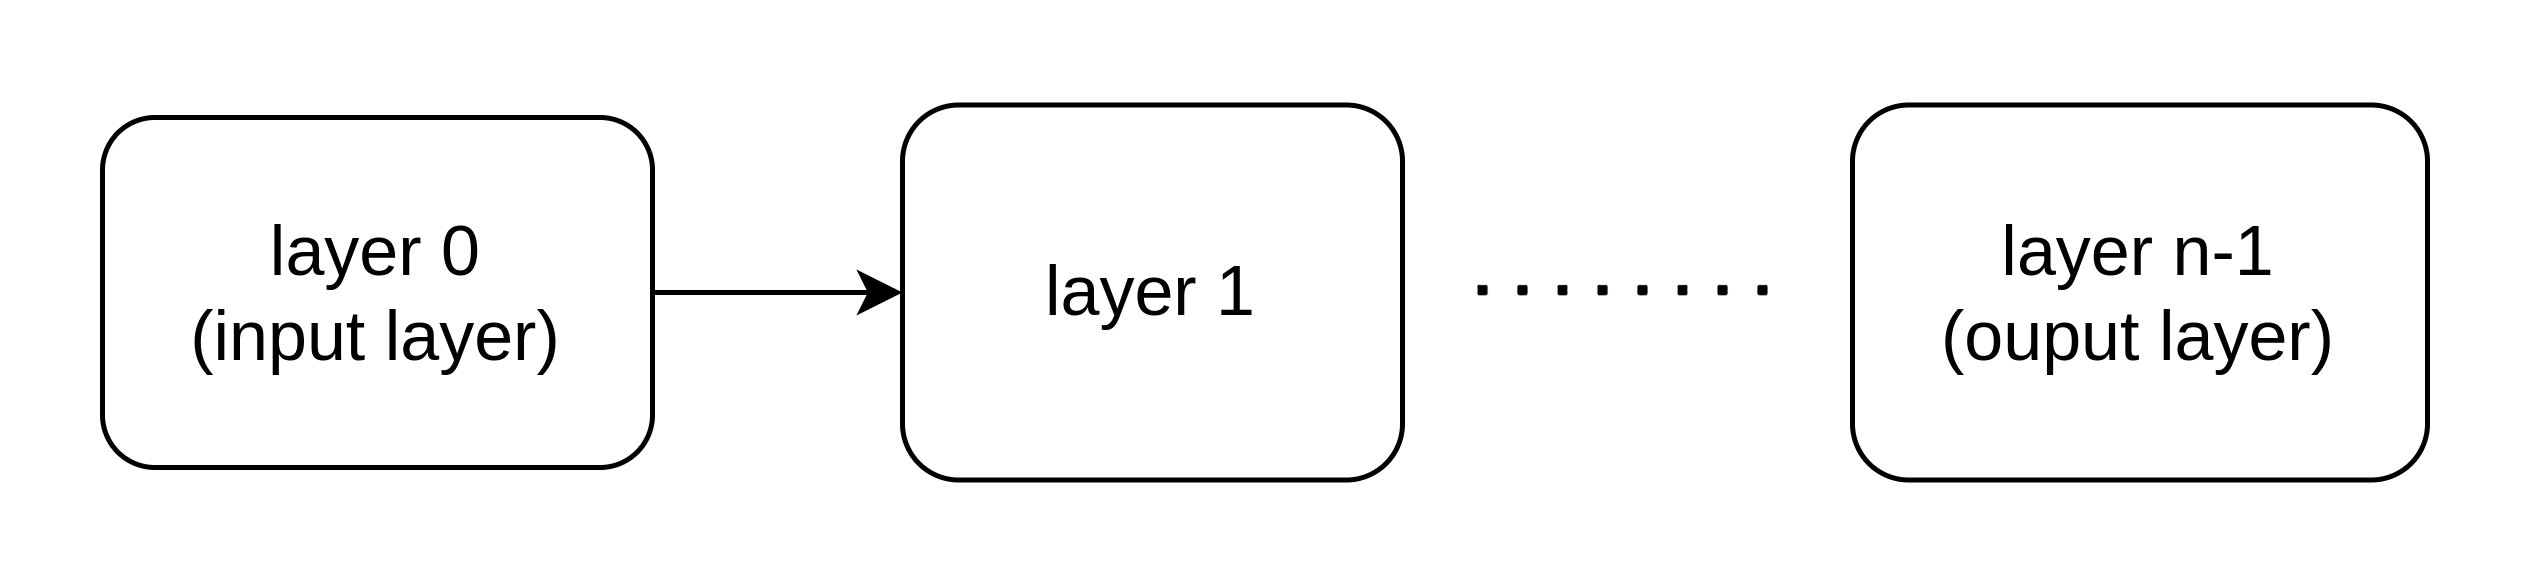
\includegraphics[width=3in]{assets/layers.png}%
\label{neural_net_arch}}
\hfil
\subfloat[]{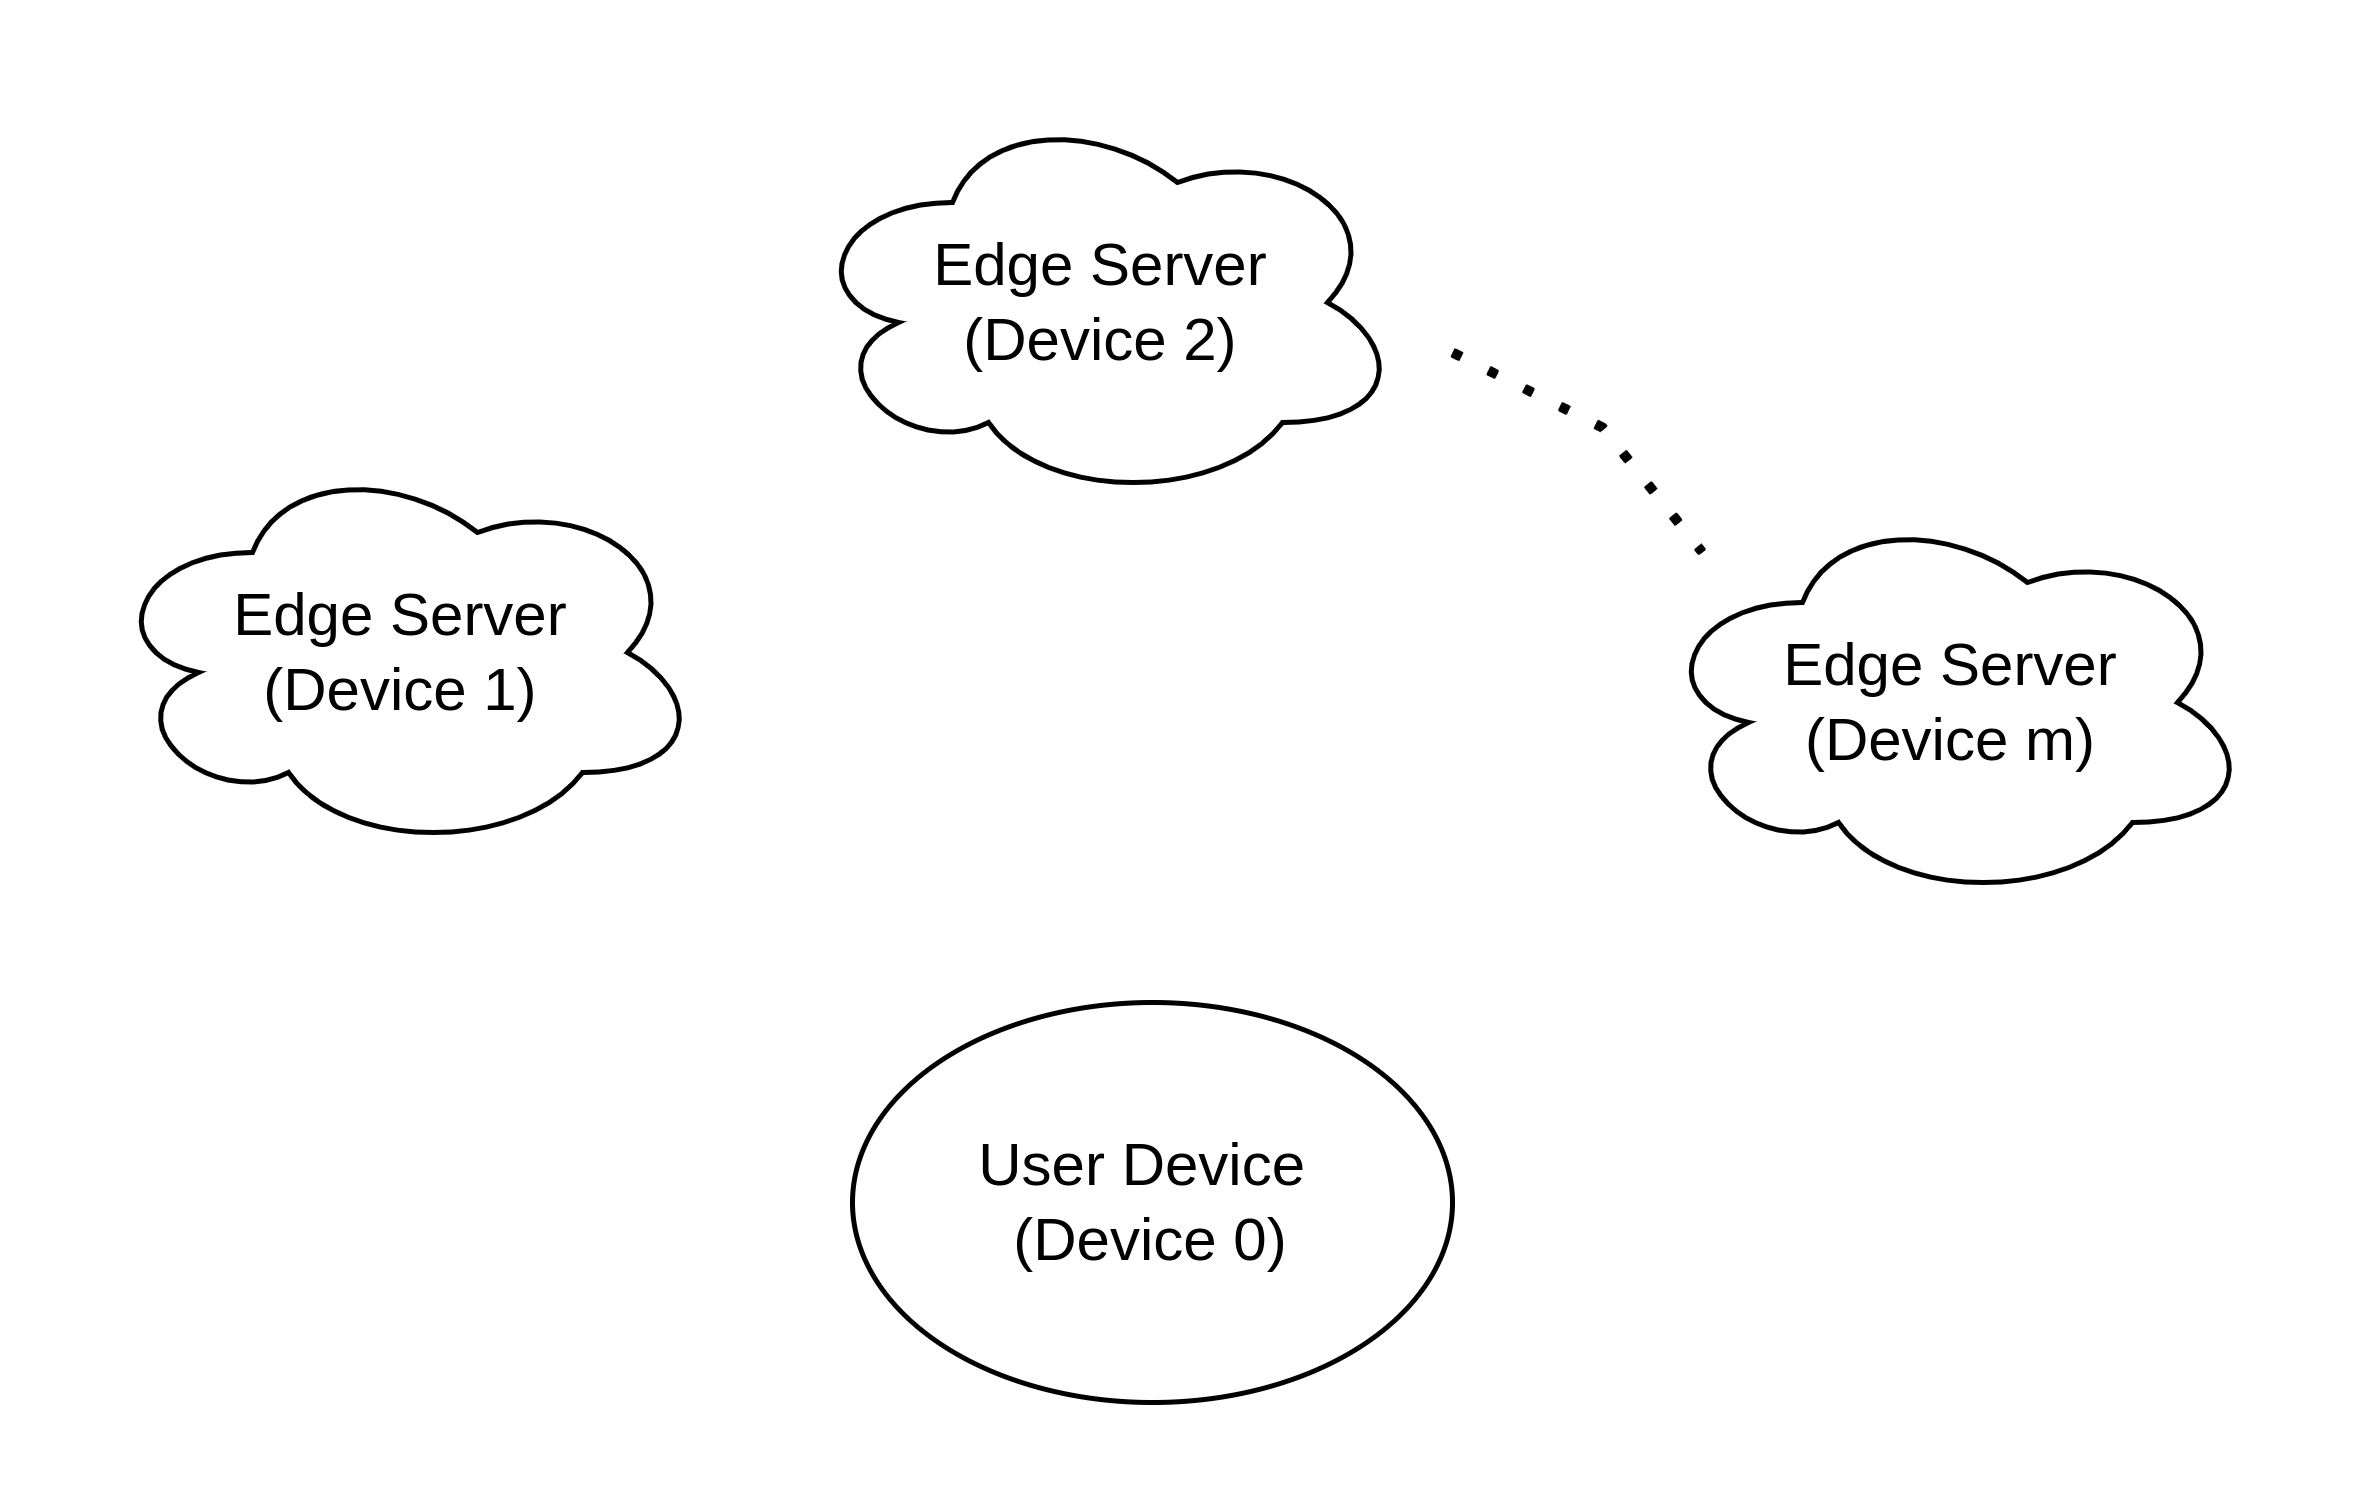
\includegraphics[width=3in]{assets/devices.png}%
\label{comp_resources}}
\caption{System model. (a) Neural network architecture. (b) Computation recources.}
\label{system_model}
\end{figure*}
System model is described in figure \ref{system_model}. We assume that neural network architecture is composed of $n$ layers. The data flow between layers is shown by a directed edge connecting the layers. Each directed edge transfers the output of one layer to the next one. Also, the output of a layer is a tensor, a generalization of matrices in a higher dimensional space. Each directed edge transfers the output of one layer to the next one. Also, the output of a layer is a tensor, a generalization of matrices in a higher dimensional space. 

Note that we assume the neural network is already partitioned, and each segment is a layer. Many algorithms can be used to partition the model graph, such as the algorithm proposed in \cite{9527097}. Thus, our purpose is to place the layers on computation resources to optimize the objective function.

Computation resources consist of $m$ edge servers and a user device. A device can run one or more layers of the model and transfer the results to another device, running the next layer of the model. However, these devices have memory limitations and a maximum number of operations per second. Furthermore, due to physical distance, transmission cost is applied between devices. Therefore, we must optimize the objective function and satisfy the constraints.

Not that, this model doesn't hold for all neural networks, as there could be multiple connections between layers. For instance, Resnet models use skip connection to deepen the network, therefore, cannot be represented by our system model.

Our objective is to minimize total inference time that consists of computation and transmission delay. First let's define input parameters of our problem:
\begin{align}
&\textbf{C} = [c]_{n(m+1)} \, : \mathrm{computation \, matrix} \, (\mathrm{operations}) \\
&\textbf{R} = [r]_{(n-1)(m+1)} \, : \mathrm{transmission \, matrix} \, (s) \\
&\boldsymbol{m_l} = [m_l]_{n} \, : \mathrm{layer \, memory \, requirement} \, (\mathrm{unit}) \\
&\boldsymbol{m_d} = [m_d]_{m+1} \, : \mathrm{device \, available \, memory} \, (\mathrm{unit}) \\
&\boldsymbol{\alpha} = [\alpha]_{m+1} \, : \mathrm{processing \, power} \, (\frac{\mathrm{operations}}{s}) \\
& K: \mathrm{maximum \, acceptable \, delay \, ratio} 
\end{align}
$c_{ij}$ element of the computation matrix corresponds to the computation cost of layer $i$ when it is placed on device $j$. Also, $r_{ij}$ element of transmission matrix denotes the transmission cost of layer $i$ output to device $j$. Note that we defined the transmission cost for each device to be independent of the layer itself. This might seem restrictive in practice, but we only consider the transmission cost that is caused by physical distance between computation devices. $\boldsymbol{m_l}$ and $\boldsymbol{m_d}$ are layer and memory requirement parameters respsectively. $\boldsymbol{\alpha}$ denotes maximum computation power of each device in number of operations per second. If the total number of layer operations in a layer is greater than its device operations, then the delay will increase to infinity. Therefore, we defined $K$ as the maximum rate of acceptable delay to limit this delay.

Define optimization variable ($X$) as:
\begin{equation}
X = [x]_{n(m+1)}, x_{ij} = \begin{cases}
1 \, , \mathrm{layer \, i \, is \, placed \, in \, device \, j} \\
0 \, , \mathrm{otherwise} \\
\end{cases}
\end{equation}
$X$ is a binary variable that makes the optimization problem a non-convex problem. Generally, these problems are NP-hard and challenging to solve.

The objective function can be expressed as:
\begin{equation}
\label{obj_func}
f_0(X) = \sum_{j=0}^{m}\sum_{i=0}^{n-1} x_{ij}\frac{c_{ij}}{\alpha_j} + \frac{1}{2}\sum_{i=0}^{n-2}\mathrm{\textbf{card}}(\boldsymbol{x}_{i+1}-\boldsymbol{x}_i)\boldsymbol{r}_i^T \boldsymbol{x}_{i+1}
\end{equation}
Note that in the objective function, $x_i$ and $r_i$ denote the row $i$ of matrix $\boldsymbol{X}$ and $\boldsymbol{R}$ respectively. First term shows the inference delay of each layer in its device. Second term is responsible for the transmission delay from one device to another. If layer $i$ and layer $i+1$ are both in the same device, then no transmission cost is applied ($\mathrm{\textbf{card}}$ will be zero). On the other hand, if two consecutive layers are in two different devices, then a transmission cost will be considered. In this case, $\mathrm{\textbf{card}}$ will be equal to $2$ and $\boldsymbol{r}_i^T \boldsymbol{x}_{i+1}$ is the transmission cost of layer $i$ to layer $i+1$. We also assume that there is no transmission cost between output layer and final user. This is the reason of iterating $i$ from 0 to $n-2$ not $n-1$.

The objective function is a non-convex as it contains cardinality operation and binary variables. Later we will satisfy these conditions and convert the objective function to a proper form. 

The objective function must be minimized while satisfying the constraints. Next, each constraint is mentioned and discussed in detail. First constraint is:
\begin{equation}
\sum_{i=0}^{n-1} c_{ij} x_{ij} \leq K \alpha_j \, , j=0, \cdots, m
\end{equation}
This constraint is responsible for limiting the maximum delay of inference on each device. Also, each layer must be assigned to only one device. Thus,
\begin{equation}
\sum_{j=0}^{m} x_{ij} = 1 \, , i=0, \cdots, n-1
\end{equation}
Finally, device memory limitations must be satisfied. Therefore,
\begin{equation}
\label{last_one}
\sum_{i=0}^{n-1} {m_l}_i x_{ij} \leq \, {m_d}_j  , j=0, \cdots, m
\end{equation}
By combining equation \ref{obj_func} to \ref{last_one}, complete form of our problem can be expressed as:
\begin{align}
\label{initial_form}
minimize &\sum_{j=0}^{m}\sum_{i=0}^{n-1} x_{ij}\frac{c_{ij}}{\alpha_j} + \frac{1}{2}\sum_{i=0}^{n-2}\mathrm{\textbf{card}}(\boldsymbol{x}_{i+1}-\boldsymbol{x}_i)\boldsymbol{r}_i^T \boldsymbol{x}_{i+1} \\
s.t. \quad & \sum_{i=0}^{n-1} c_{ij} x_{ij} \leq K \alpha_j \, , j \in [0, m] \nonumber \\
\quad & \sum_{j=0}^{m} x_{ij} = 1 \, , i \in [0, n-1] \nonumber \\
\quad & \sum_{i=0}^{n-1} {m_l}_i x_{ij} \leq \, {m_d}_j  , j \in [0, m] \nonumber \\
\quad & x_{ij} \in \{0,1\} \, , i \in [0, n-1]; \, j \in [0, m] \nonumber
\end{align}
\subsection{Approximation and Conversion}
In this section, problem \ref{initial_form} will be approximated and converted to a simpler form, so that it can be solved by general solvers. First of all, we approximate $\mathrm{\textbf{card}}$ function with L1 norm. Therefore, $\mathrm{\textbf{card}}(\boldsymbol{x}_{i+1}-\boldsymbol{x}_i)$ can be replaced with $\sum_{j=0}^{m} |x_{(i+1)j}-x_{ij}|$ function. Also, this term can be replaced with another binary variable and adding two sets of constraints to the original problem. The main idea is to define a new binary variable $y_{ij}$ to replace $|x_{(i+1)j}-x_{ij}|$ while it satisfies $x_{(i+1)j}-x_{ij} \leq y_{ij}$ and $x_{(i+1)j}-x_{ij} \geq -y_{ij}$. Therefore, the approximated form of optimization problem becomes:
\begin{align}
minimize &\sum_{j=0}^{m}\sum_{i=0}^{n-1} x_{ij}\frac{c_{ij}}{\alpha_j} + \frac{1}{2}\sum_{i=0}^{n-2} \sum_{j=0}^{m} y_{ij} r_{ij} x_{(i+1)j} \\
s.t. \quad & \sum_{i=0}^{n-1} c_{ij} x_{ij} \leq K \alpha_j \, , j \in [0, m] \nonumber \\
\quad & \sum_{j=0}^{m} x_{ij} = 1 \, , i \in [0, n-1] \nonumber \\
\quad & \sum_{i=0}^{n-1} {m_l}_i x_{ij} \leq \, {m_d}_j  , j \in [0, m] \nonumber \\
\quad & x_{(i+1)j}-x_{ij} \leq y_{ij} \, , i \in [0, n-2]; \, j \in [0,m]  \nonumber \\
\quad & x_{(i+1)j}-x_{ij} \geq -y_{ij} \, , i \in [0, n-2]; \, j \in[0,m]  \nonumber \\
\quad & x_{ij} \in \{0,1\} \, , i \in [0, n-1]; \, j \in [0,m] \nonumber \\
\quad & y_{ij} \in \{0,1\} \, , i \in [0, n-2]; \, j \in [0,m] \nonumber
\end{align}
The approximated problem is clearly a quadratic integer (binary) programming problem. Quadratic form can be expressed as $z^TQz$ which $Q$ is a symmetric matrix with all zero on its main diagonal. Due to the non-positive semi-definite nature of this matrix, we cannot use a more general solver. Furthermore, most solvers can deal with mixed-integer linear programming problems but fail to solve an integer problem with the quadratic form. Hence, we simplify this problem further by converting it to a binary (integer) programming problem, which can be solved by various optimization techniques. 

The main idea is to introduce more binary variables that replace the $y_{ij}x_{(i+1)j}$ product. The product of two binary variables is also a binary variable. Therfore, by defining $w_{ij} = x_{(i+1)j}y_{ij} \, , i=0,\cdots,n-2 \, , j=0,\cdots,m$, objective function can be converted to a linear form. Also two set of constraints are added to the approximated problem. If $x_{(i+1)j} = 0$, then $w_{ij} = 0$ too. This is a forcing constraint which is a linear constraint. The same relationships hold for $y_{ij}$, too. Also, if both $x_{(i+1)j}$ and $y_{ij}$ equal to $1$, then $w_{ij} = 1$ too. Finally, by combining these modifications, our optimization problem can be expressed as:
\begin{align}
\label{final_form}
minimize &\sum_{j=0}^{m}\sum_{i=0}^{n-1} x_{ij}\frac{c_{ij}}{\alpha_j} + \frac{1}{2}\sum_{j=0}^{m} \sum_{i=0}^{n-2} w_{ij} r_{ij} \\
s.t. \quad & \sum_{i=0}^{n-1} c_{ij} x_{ij} \leq K \alpha_j \, , j \in [0, m] \nonumber \\
\quad & \sum_{j=0}^{m} x_{ij} = 1 \, , i \in [0, n-1] \nonumber \\
\quad & \sum_{i=0}^{n-1} {m_l}_i x_{ij} \leq \, {m_d}_j  , j \in [0, m] \nonumber \\
\quad & x_{(i+1)j}-x_{ij} \leq y_{ij} \, , i \in [0, n-2]; \, j \in [0,m]  \nonumber \\
\quad & x_{(i+1)j}-x_{ij} \geq -y_{ij} \, , i \in [0, n-2]; \, j \in[0,m]  \nonumber \\
\quad & z_{ij} \leq y_{ij} \, , i \in [0, n-2]; \, j \in [0, m]  \nonumber \\
\quad & z_{ij} \leq x_{(i+1)j} \, , i \in [0, n-2]; \, j \in [0, m]  \nonumber \\
\quad & z_{ij} \geq x_{(i+1)j} + y_{ij} - 1 \, , i \in [0, n-2]; \, j \in [0, m]  \nonumber \\
\quad & x_{ij} \in \{0,1\} \, , i \in [0, n-1]; \, j \in [0,m] \nonumber \\
\quad & y_{ij}, w_{ij} \in \{0,1\} \, , i \in [0, n-2]; \, j \in [0,m] \nonumber
\end{align}
We ended up having a binary linear programming problem that most solvers can solve. This conversion involves a trade-off between increasing the optimization space's dimension and simplifying the problem. We increased the number of variables with the cost of solving the problem easily and having a simpler form.

\section{Simulation}
To solve this problem and simulate it, problem \ref{final_form} is represented in matrix and vector format. The detail of this representation is not discussed in this section, but you can refer to simulation code for more information. Equivalent form in matrix format is,
\begin{align}
\label{matrix_form}
minimize \, \, & \boldsymbol{p}^T \boldsymbol{z} + \boldsymbol{q}^T \boldsymbol{w} \\
s.t.  \, \, & \boldsymbol{S_1} \boldsymbol{z} \leq 0 \, , \quad -\boldsymbol{S_2} \boldsymbol{z} \leq 0 \nonumber \\
\quad & \boldsymbol{L}\boldsymbol{z} \leq \boldsymbol{h} \nonumber \\
\quad &  \boldsymbol{E} \boldsymbol{z} = \boldsymbol{1}_{n}  \nonumber \\
\quad &  \boldsymbol{M} \boldsymbol{z} \leq \boldsymbol{M_d} \nonumber \\
\quad &  \boldsymbol{U} \boldsymbol{z} + \boldsymbol{w} \leq 0 \, , \boldsymbol{V} \boldsymbol{z} + \boldsymbol{w} \leq 0 \nonumber \\
\quad &  \boldsymbol{G} \boldsymbol{z} - \boldsymbol{w} \leq \boldsymbol{1}_{(m+1)(n-1)} \nonumber \\
\quad &  \boldsymbol{z} \in \{0, 1\}^{(m+1)(2n-1)} \, , \boldsymbol{w} \in \{0, 1\}^{(m+1)(n-1)} \nonumber
\end{align}
In this problem, $\boldsymbol{z}$ and $\boldsymbol{w}$ are optimization variables. Other parameters are derived from problem parameters and equation \ref{final_form}. 

We simulated this problem with the following input parameters:
\begin{align}
&m = 2, \, n = 3, \, K = 2 \, , \boldsymbol{C} = \begin{bmatrix}
100 & 200 & 200 \\
100 & 200 & 200 \\
100 & 200 & 200
\end{bmatrix} \\
&\boldsymbol{R} = \begin{bmatrix}
10 & 20 & 30 \\
10 & 20 & 30
\end{bmatrix} \, , \boldsymbol{m_l} = \begin{bmatrix}
100 & 100 & 300
\end{bmatrix} \, , \nonumber \\
&\boldsymbol{m_d} = \begin{bmatrix}
500 & 500 & 500
\end{bmatrix} \, , \boldsymbol{\alpha} = \begin{bmatrix}
50 & 60 & 100 \nonumber
\end{bmatrix}
\end{align}
We choosed a simple problem to show the concept of our approach. We used cvxpy and MOSEK to solve this problem. MOSEK is a commersial optimization tool that can handle large scale problems efficiently. The simulation code is sent along with this report. Also, whole content of project can be accesed thorugh \href{https://github.com/NimaSamadi007/cvxopt2-project}{this github repository}. To run the simulation. you need cvxpy, numpy and MOSEK license. 

It's obvious that all 3 layers must be placed on last device (edge server 2) as it eliminates the transmission cost and can handle all layers simultaneously. The total delay in this case is $\mathrm{delay} = \frac{200}{100}+\frac{200}{100}+\frac{200}{100}=6$ and is optimal. When simulation is run, the following result is achieved:
\begin{figure}[H]
\centering
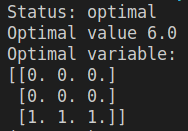
\includegraphics[width=1.5in]{assets/opt-res.png}
\caption{Simulation result}
\end{figure}
Which proves our observation. Note that our main objective in this project was to formulate this problem in a simple form not simulation. However, we run the simulation to show the correctness of our formulation. 
\section{Conclusion}
In this project, we investigated a DNN model placement problem with an optimization approach. DNN models are at the heart of edge intelligence and running these models efficiently is an important problem. We formulated the problem as a linear binary programming problem that can be solved with various optimization techniques, such as branch and bound. Also, a simulation of a simple scenario was done with MOSEK, and the results were discussed. Our contributions can be summarized as follows:
\begin{enumerate}
\item{Optimization approaches were applied to an industrial problem}
\item{Defining a hyperparameter to control maximum inference time of the model in total ($K$)}
\item{Approximation of the original problem and converting it to a linear form}
\item{Simulation of the problem with MOSEK}
\end{enumerate}
Some of the assumptions in this project can be relaxed in future works. DNN model can be generalized to include more sophisticated architectures. Transmission cost between devices must also be a function of the current layer. More simulations must be done and timing results must be compared.

\bibliographystyle{IEEEtran}
\bibliography{IEEEabrv,citation.bib}
\end{document}
